\subsection{Сильное и слабое кристаллическое поле. Магнитные и спектральные свойства комплексных соединений переходных металлов}

 Лиганды делятся на две группы – сильного поля, которые расщепляют сильно-низкоспиновые комплексы, и лиганды слабого поля-высокоспиновые комплексы, которые расщепляют слабо. 
 
Интенсивность поля возрастает в следующем ряду:
 
\begin{figure}[H]
\centering
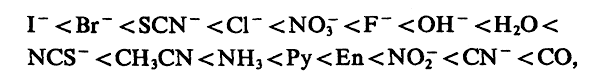
\includegraphics[scale=.600]{images/spectrochem_row.png}
\end{figure}
 
 \subsubsection{Октаэдрическое поле}
 
 \begin{figure}[htp]
\centering
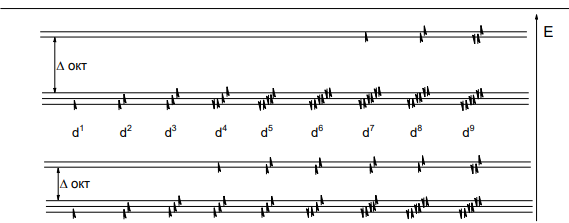
\includegraphics[scale=1.00]{images/electrones.png}
\end{figure} схема заполнения электронов представлена на картинке

 \begin{itemize}
 \item для $d^1-d^3$ ситуация не зависит от расщепления \item для $d^4$ ситуация меняется есть два варианта: для слабого(нижняя диаграмма) расщепления разница в энергии невелика и электроны остаются неспаренными. Образуются 4 неспаренных электрона  для сильного расщепления разница в энергии уровней больше чем энергии спаривания, поэтому получается выигрыш в энергии, когда электрон опускается вниз и спариваются \item для $d^5$ в низкоспиновом комплексе 2 спаренных электрона и 1 неспаренный в высокоспиновом комплексе пять неспаренных электронов для $d^6$ в низкоспиновом комплексе получится полностью заполненные $d_{xz}$,$d_{xy}$,$d_{yz}$ орбитали-диамагнитный комплекс в высокоспиновом комплексе 4 неспаренных электрона 
 \item для $d^7$ в низкоспиновом комплексе 1 неспаренный электрон в высокоспиновом комплексе 3 неспаренных электрона 
 \item для $d^8$-$d^9$ в низкоспиновом комплексе и в высокоспиновом комплексе будут одинаковые картины- по 2(для $d^8$) и 3( для $d^9$) электронов 
 \end{itemize}

\subsubsection*{Тетраэдрическое поле}
тетраэрдрические комплексы формируются только лиганды со слабым полем(высокоспиновые)-почему? потому что $0.5\Delta_{oct}=\Delta_{tetr}$ ( расщепление мало) и спариваться электронам не нужно

а почему расщепление меньше?
\begin{itemize}
\item расстояние до лигандов в тетраэдрическом поле больше, взаимодействие хуже 
\item количество лигандов меньше, чем в окаэдрическом поле и поэтому отталкивание меньше энергия спаривания электронов ($P$) больше, чем $10D_q$ и первые 5 электронов заполняют по одному пять орбиталей и шестой(и последующие) электроны с обратным спином дополняют каждую орбитали. 
\end{itemize}

\subsubsection{магнитные свойства}
 магнитный момент у низкоспиновых меньше, так как электроны спариваются, а не переходят на другие уровни 
$$\mu=2\sqrt{s(s+1)}=\sqrt{n(n+2)}$$ 

s-суммарный спин 

n-число неспаренных электронов 

\subsubsection{Спектральные свойства}
 В зависимости от лигандов комплекс имеет разные цвета. При замещении лиганда изменяется не только число неспаренных электронов, но еще и цвет. В случае высокоспинового комплекса энергия расщепления меньше($E=h\nu$), следовательно частота перехода с $d_{xy},d_{xz},d_{yz}$ на $d_z^2$ , $d_x^2-d_y^2$ меньше, а длина волны поглощаемого цвета больше В случае низкоспинового комплекса ситуация обратная, энергия расщепления больше($E=h\nu$), следовательно частота перехода сс $d_{xy},d_{xz},d_{yz}$ на $d_z^2$ , $d_x^2-d_y^2$ больше, а длина волны поглощаемого цвета меньше (будет поглощать более коротковолновые волны) \begin{figure}[htp]
 
\subsubsection{Соответствие частот и цветов}
\centering
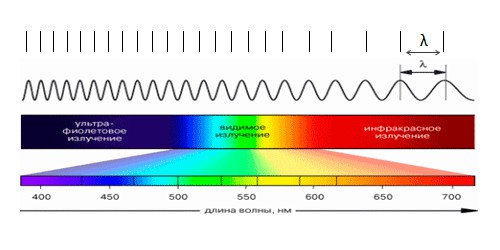
\includegraphics[scale=.750]{images/spectre.jpg}
\end{figure}
 
 